\section{First Part (ViolaJones):}
The code for Viola Jones is made up of the following files
\begin{itemize}
	\item \textbf{ConvertHaarcasadeXMLOpenCV.m}: This function is required to translate OpenCV feature functions from XML to syntax Matlab can understand.
	\item \textbf{ObjectDetection.m}: This is the beginning of the detection where the input parameters are received and the function to return the \textbf{Rectangle} matrices is called. 	
	\item \textbf{GetIntergralImages.m}: This function computes the \textbf{integral matrix} for the image.
\end{itemize}

\subsection{Code:}
\noindent Let's start by describing what is important about the codes:\\
\noindent The first code called would be \textbf{ObjectDetection.m} Listing \ref{lst:ObjectDetection}:\\
\noindent On line 3 of the Listing \ref{lst:ObjectDetection}, we have the default options:
\begin{itemize}
	\item \textbf{ScaleUpdate}: This tells us that the scale of the current \textbf{window} will increase from 1 to 1.2 in each iteration, that is, if the current scale is $X$, the next scale will be $1.2X$. 
	\item \textbf{Resize}: Resizes the image so that the longest side (width or height) is equal to 384.
	\item \textbf{Verbose}: this is to show the calculations of the iterations.
\end{itemize}

\noindent On line 31 of the Listing \ref{lst:ObjectDetection}, here we load the image and convert it into an array, but if the image is color then the pixes of the array has 3 values in eache pixel (r,g,v).\\

\noindent On line 35 of the Listing \ref{lst:ObjectDetection}, this function extracts the feature functions already trained by \textbf{OpenCV}, which are our \textbf{Strong Classifiers} when examining each \textbf{window}, as shown in class slide Figure \ref{fig:slideT1}.\\

\noindent On line 37 of the Listing \ref{lst:ObjectDetection},we compute the \textbf{integral matrix} using the function \textbf{GetIntergralImages.m} (see Listing \ref{lst:GetIntergralImages})\\

\noindent On line 1 of the Listing \ref{lst:GetIntergralImages}, we convert the image array to a double-type.\\

\noindent On lines from 2 to 12 of the Listing \ref{lst:GetIntergralImages}, the image resize mentioned is performed (option resize) and the reason for the ratio between the real size of the image and its current size is saved $Ratio=size(Picture,2)/384$.\\


\begin{lstlisting}[style=Matlab-editor, numbers=left,label={lst:GetIntergralImages},captionpos=b, caption={Code \textbf{GetIntergralImages.m} }]
Picture=im2double(Picture);

if(Options.Resize)
if (size(Picture,2) > size(Picture,1)),
	Ratio = size(Picture,2) / 384;
else
	Ratio = size(Picture,1) / 384;
end
	Picture = imresize(Picture, [size(Picture,1) size(Picture,2) ]/ Ratio);
else
	Ratio=1;
end

if(size(Picture,3)>1),
	Picture=0.2989*Picture(:,:,1) + 0.5870*Picture(:,:,2)+ 0.1140*Picture(:,:,3);
end

s=zeros([size(Picture,1),size(Picture,2)]);
ii=zeros([size(Picture,1),size(Picture,2)]);
for x=1:size(Picture,1)
	for y=1:size(Picture,2)
		if(x==1 && y==1)
			s(x,y)=Picture(x,y);
			ii(x,y)=s(x,y);
		elseif(x==1 && y>1)
			s(x,y)=s(x,y-1)+Picture(x,y);
			ii(x,y)=s(x,y);
		elseif(x>1 && y==1)
			s(x,y)=Picture(x,y);
			ii(x,y)=ii(x-1,y)+s(x,y);
		else
			s(x,y)=s(x,y-1)+Picture(x,y);
			ii(x,y)=ii(x-1,y)+s(x,y);
		end
	end
end
IntegralImages.ii=ii;

IntegralImages.ii=padarray(IntegralImages.ii,[1 1], 0, 'pre');

s2=zeros([size(Picture,1),size(Picture,2)]);
ii2=zeros([size(Picture,1),size(Picture,2)]);
for x=1:size(Picture,1)
	for y=1:size(Picture,2)
		if(x==1 && y==1)
			s2(x,y)=Picture(x,y)^2;
			ii2(x,y)=s(x,y);
		elseif(x==1 && y>1)
			s2(x,y)=s(x,y-1)+Picture(x,y)^2;
			ii2(x,y)=s(x,y);
		elseif(x>1 && y==1)
			s2(x,y)=Picture(x,y)^2;
			ii2(x,y)=ii2(x-1,y)+s2(x,y);
		else
			s2(x,y)=s2(x,y-1)+Picture(x,y)^2;
			ii2(x,y)=ii2(x-1,y)+s2(x,y);
		end
	end
end
IntegralImages.ii2=ii2;

IntegralImages.ii2=padarray(IntegralImages.ii2,[1 1], 0, 'pre');

IntegralImages.width = size(Picture,2);
IntegralImages.height = size(Picture,1);
IntegralImages.Ratio=Ratio;
\end{lstlisting}


\begin{lstlisting}[style=Matlab-editor, numbers=left,label={lst:ObjectDetection},captionpos=b, caption={Code \textbf{ObjectDetection.m} }]
	function Objects = ObjectDetection(Picture,FilenameHaarcasade,Options)
	
	defaultoptions=struct('ScaleUpdate',1/1.2,'Resize',true,'Verbose',true);
	
	functionname='ObjectDetection.m';
	functiondir=which(functionname);
	functiondir=functiondir(1:end-length(functionname));
	addpath([functiondir '/SubFunctions'])

	if(ischar(Picture))
		if(~exist(Picture,'file'))
			error('face_detect:inputs','Image not Found');
		end
	end
	if(~exist(FilenameHaarcasade,'file'))
		error('face_detect:inputs','Haarcasade not Found');
	end

	if(~exist('Options','var')), Options=defaultoptions;
	else
		tags = fieldnames(defaultoptions);
		
	for i=1:length(tags),
		if(~isfield(Options,tags{i})), Options.(tags{i})=defaultoptions.(tags{i}); end
	end
		if(length(tags)~=length(fieldnames(Options))),
			warning('image_registration:unknownoption','unknown options found');
		end
	end

	if(ischar(Picture))
		Picture = imread(Picture);
	end

	HaarCasade=GetHaarCasade(FilenameHaarcasade);

	IntergralImages= GetIntergralImages(Picture,Options);
	
	Objects = HaarCasadeObjectDetection(IntergralImages,HaarCasade,Options);

	if(nargout==0)
		ShowDetectionResult(Picture,Objects);
	end
\end{lstlisting}

\begin{figure}[h]
	\centering
	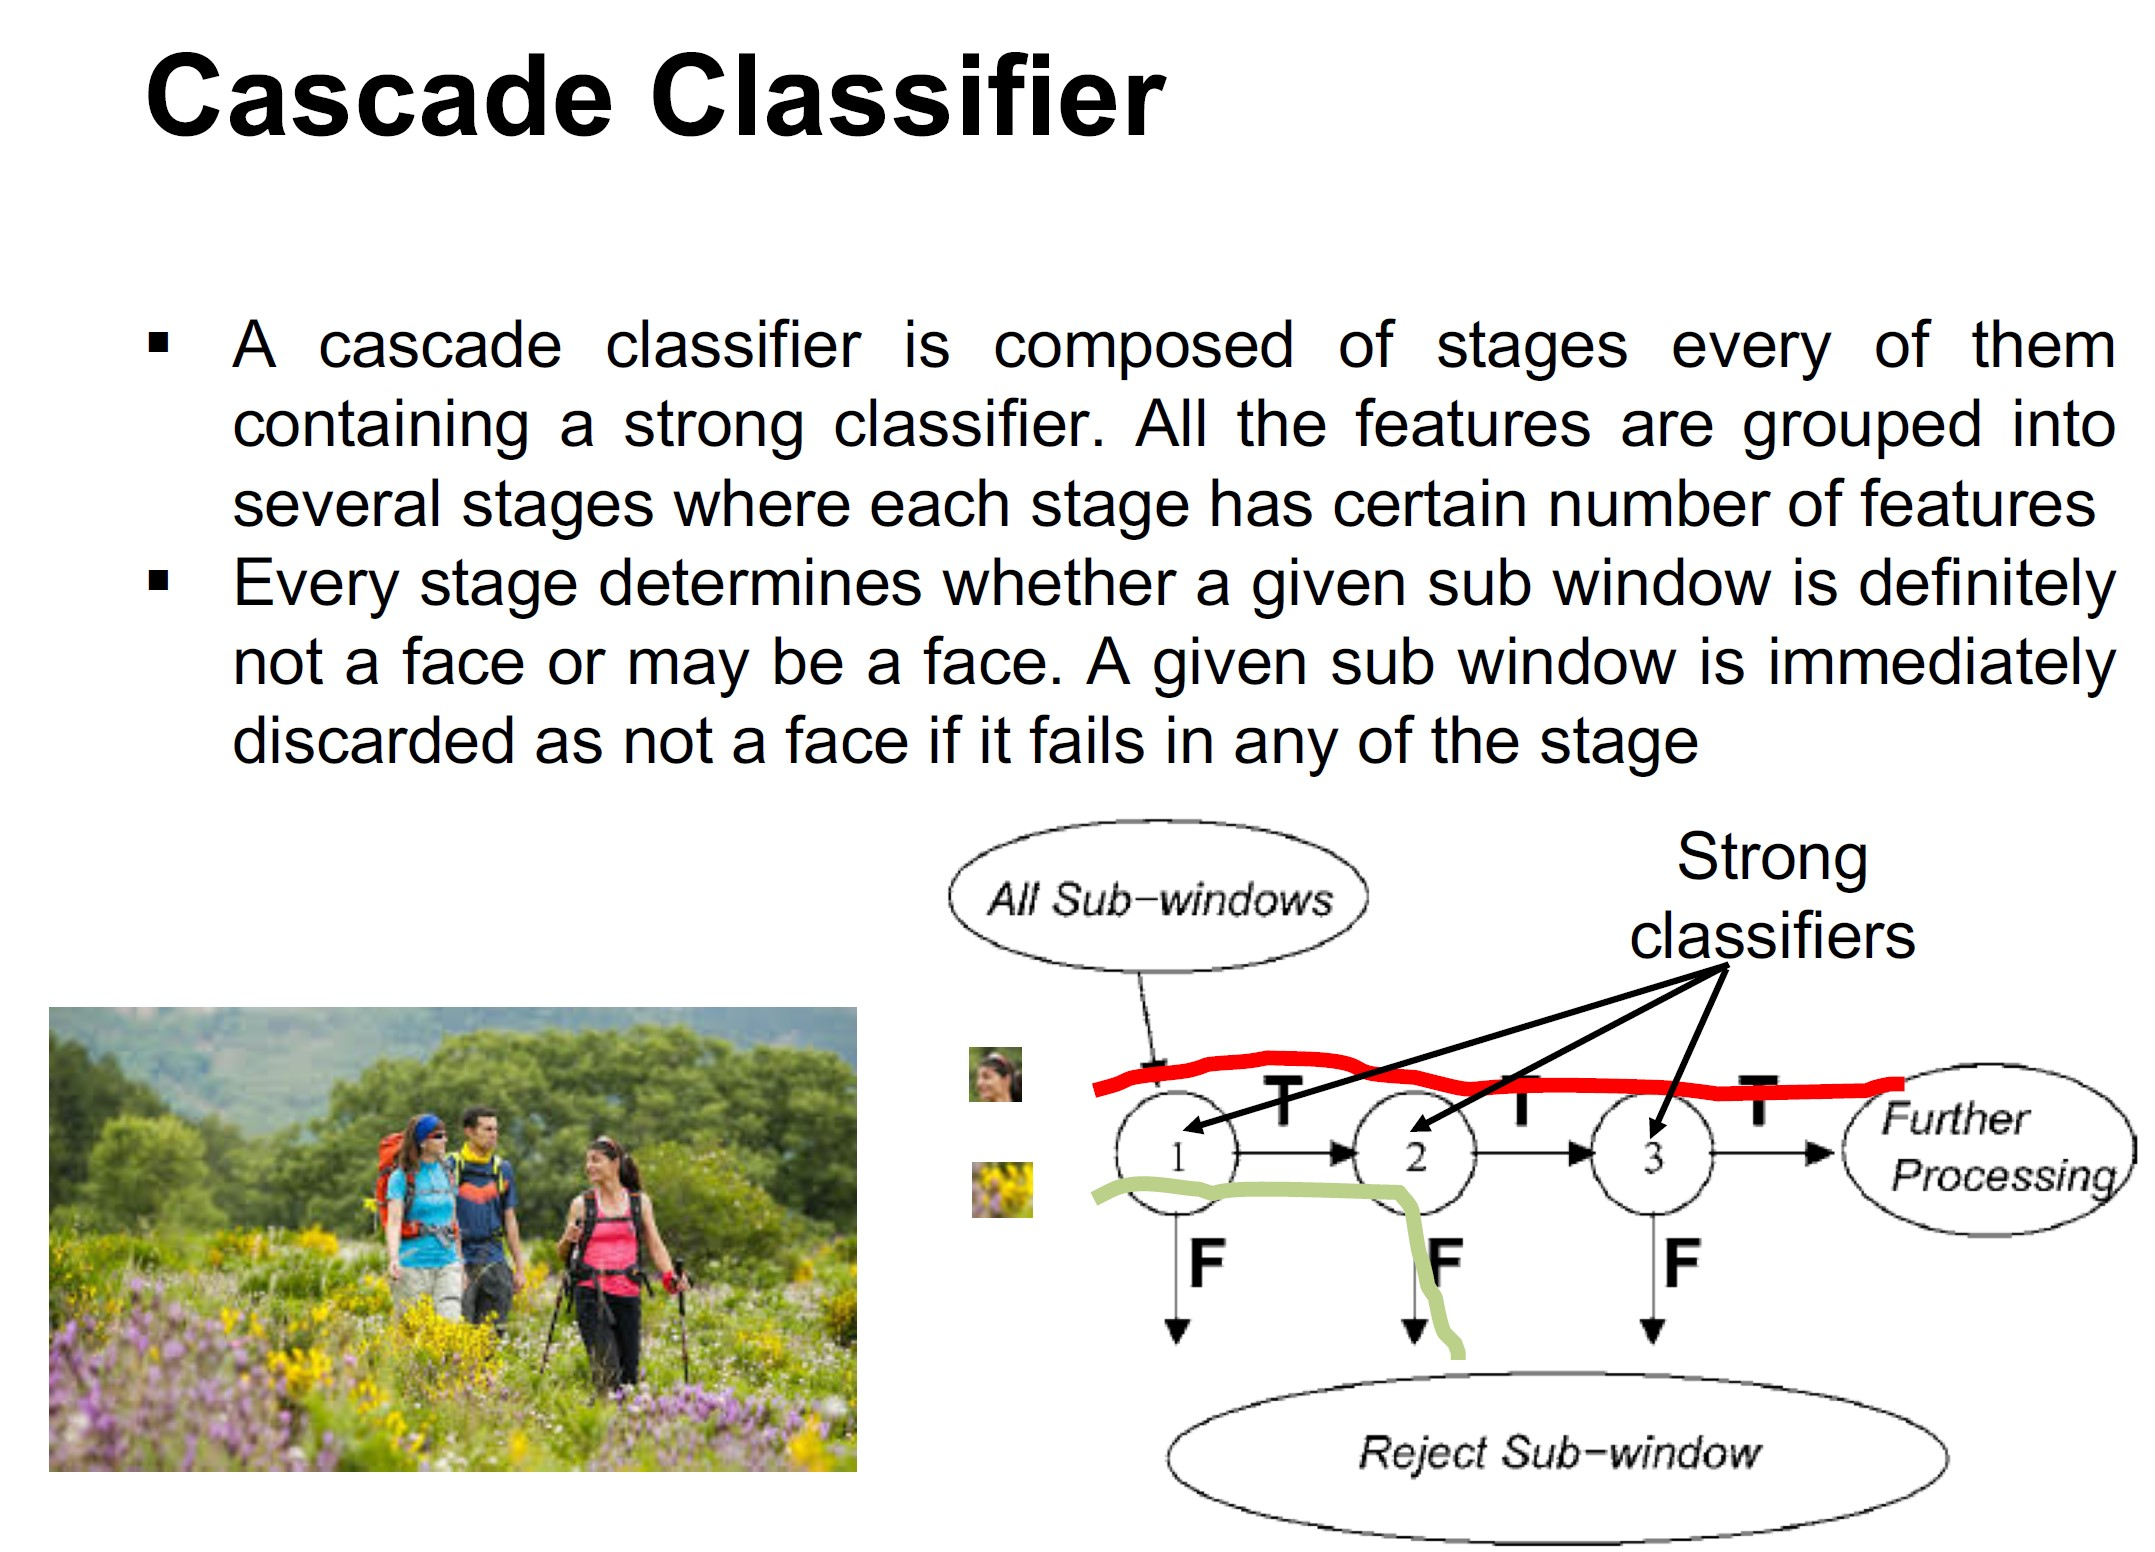
\includegraphics[width=0.75\textwidth]{T1/classifier}
	\caption{Cascade Classifier}
	\label{fig:slideT1}
\end{figure}